\documentclass[aspectratio=169]{beamer}

% ── Thème ──────────────────────────────────────────────────────────────
\usetheme{Madrid}
\definecolor{primary}{RGB}{67,97,238}
\definecolor{secondary}{RGB}{114,9,183}
\definecolor{accent}{RGB}{76,201,240}
\definecolor{lightbg}{RGB}{241,245,249}

\setbeamercolor{palette primary}{bg=primary,fg=white}
\setbeamercolor{palette secondary}{bg=primary!80,fg=white}
\setbeamercolor{palette tertiary}{bg=primary!60,fg=white}
\setbeamercolor{palette quaternary}{bg=primary,fg=white}
\setbeamercolor{structure}{fg=primary}
\setbeamercolor{section in toc}{fg=primary}
\setbeamercolor{frametitle}{bg=primary,fg=white}
\setbeamercolor{block title}{bg=primary,fg=white}
\setbeamercolor{block body}{bg=lightbg}
\setbeamercolor{alerted text}{fg=secondary}
\setbeamercolor{alertblock title}{bg=secondary,fg=white}

% ── Packages ─────────────────────────────────────────────────────────────
\usepackage[utf8]{inputenc}
\usepackage[T1]{fontenc}
\usepackage[french]{babel}
\usepackage{graphicx}
\usepackage{tikz}
\usepackage{fontawesome5}
\usepackage{xcolor}
\usepackage[export]{adjustbox}

\graphicspath{{chapters/assets/images/}}

% ── Footline ─────────────────────────────────────────────────────────────
\setbeamertemplate{navigation symbols}{}
\setbeamertemplate{footline}{
  \leavevmode\hbox{
    \begin{beamercolorbox}[wd=.33\paperwidth,ht=2.25ex,dp=1ex,center]{author in head/foot}
      \usebeamerfont{author in head/foot}Abdelghani Saidi
    \end{beamercolorbox}
    \begin{beamercolorbox}[wd=.34\paperwidth,ht=2.25ex,dp=1ex,center]{title in head/foot}
      \usebeamerfont{title in head/foot}My Smart Budget · PFE 2026
    \end{beamercolorbox}
    \begin{beamercolorbox}[wd=.33\paperwidth,ht=2.25ex,dp=1ex,right]{date in head/foot}
      \usebeamerfont{date in head/foot}\insertframenumber{} / \inserttotalframenumber\hspace*{1em}
    \end{beamercolorbox}
  }
}

% ── Commande utilitaire : image pleine slide ──────────────────────────────
% Usage : \fullimg{fichier}{légende}
\newcommand{\fullimg}[2]{%
  \begin{frame}{#2}
    \begin{center}
      \includegraphics[max width=\linewidth, max height=0.82\textheight, keepaspectratio]{#1}
    \end{center}
  \end{frame}
}

% ── Métadonnées ──────────────────────────────────────────────────────────
\title[PFE : My Smart Budget]{\textbf{My Smart Budget}}
\subtitle{Conception et développement d'une application web\\de gestion budgétaire personnelle}
\author[Abdelghani Saidi]{Abdelghani Saidi}
\institute{Projet de Fin d'Études}
\date{2026}

% ═════════════════════════════════════════════════════════════════════════
\begin{document}
% ═════════════════════════════════════════════════════════════════════════

% ── TITRE ────────────────────────────────────────────────────────────────
{
\setbeamertemplate{footline}{}
\begin{frame}
  \begin{tikzpicture}[remember picture,overlay]
    \fill[primary] (current page.north west) rectangle (current page.south east);
    \fill[secondary!50,opacity=0.25] (current page.north east) circle (7cm);
    \fill[accent!40,opacity=0.18] (current page.south west) circle (5cm);
  \end{tikzpicture}
  \vspace{1.2cm}
  \titlepage
\end{frame}
}

% ── PLAN ─────────────────────────────────────────────────────────────────
\begin{frame}{Plan}
  \tableofcontents
\end{frame}

% ═════════════════════════════════════════════════════════════════════════
\section{Présentation du projet}
% ═════════════════════════════════════════════════════════════════════════

\begin{frame}{My Smart Budget — Vue d'ensemble}
  \begin{columns}[t]
    \begin{column}{0.48\textwidth}
      \begin{block}{Contexte}
        Application web de \textbf{gestion budgétaire personnelle} pour aider l'utilisateur à suivre ses finances et atteindre ses objectifs d'épargne.
      \end{block}
      \vspace{0.4cm}
      \begin{block}{Stack technique}
        \begin{itemize}
          \item \textbf{Frontend :} Next.js · TypeScript · Tailwind
          \item \textbf{Backend :} Node.js · Express · API REST
          \item \textbf{BDD :} PostgreSQL 15 · MongoDB
          \item \textbf{Auth :} JWT · Cookies HTTPOnly
        \end{itemize}
      \end{block}
    \end{column}
    \begin{column}{0.48\textwidth}
      \begin{block}{Fonctionnalités principales}
        \begin{itemize}
          \item[\textcolor{accent}{\faCheck}] Tableau de bord financier
          \item[\textcolor{accent}{\faCheck}] Gestion des transactions
          \item[\textcolor{accent}{\faCheck}] Enveloppes budgétaires
          \item[\textcolor{accent}{\faCheck}] Objectifs d'épargne
          \item[\textcolor{accent}{\faCheck}] Export RGPD (PDF / JSON)
          \item[\textcolor{accent}{\faCheck}] Alertes de dépassement
        \end{itemize}
      \end{block}
    \end{column}
  \end{columns}
\end{frame}

% ═════════════════════════════════════════════════════════════════════════
\section{Analyse des besoins}
% ═════════════════════════════════════════════════════════════════════════

\begin{frame}{Profils utilisateurs ciblés}
  \begin{columns}[c]
    \begin{column}{0.31\textwidth}
      \centering
      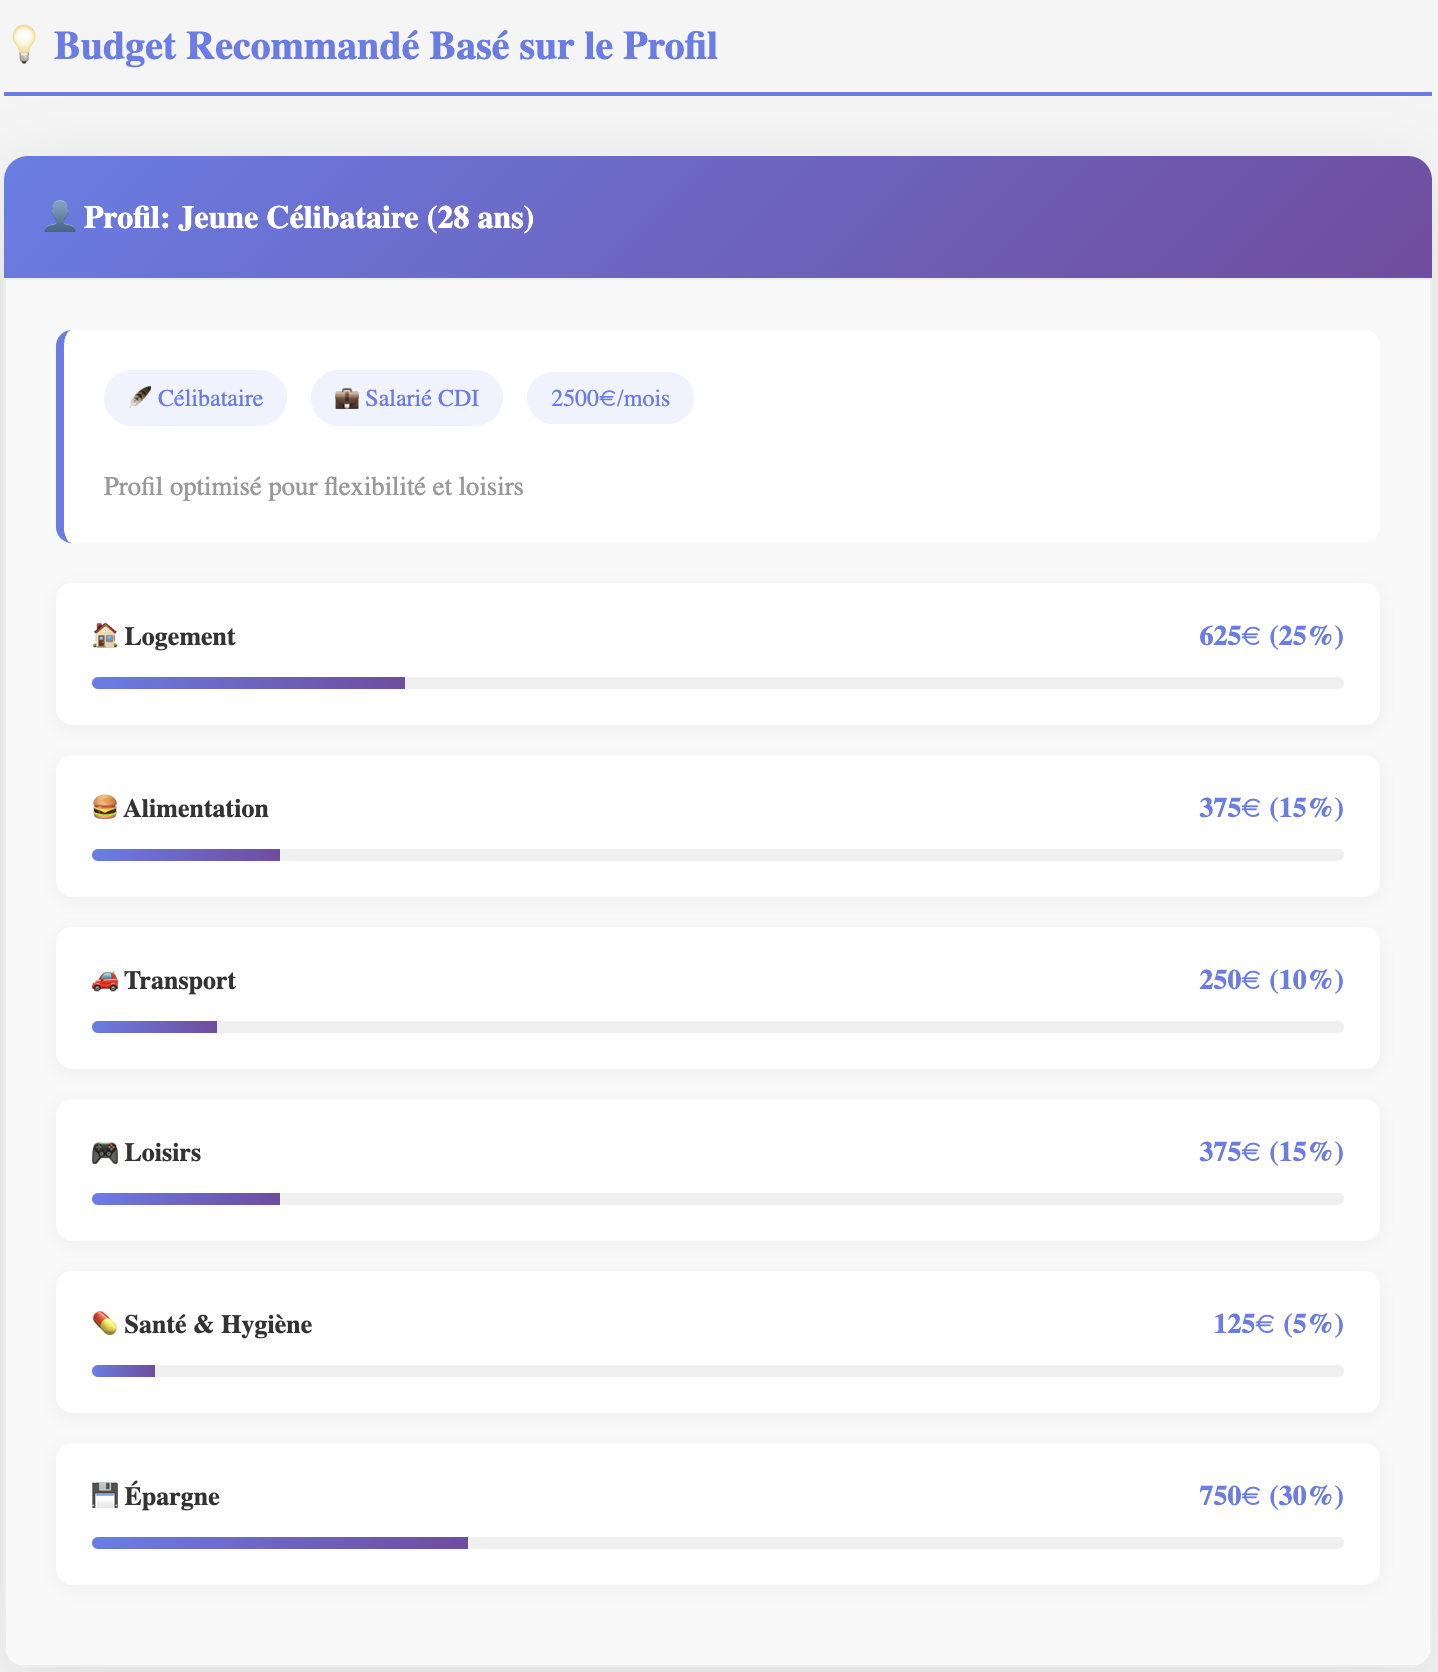
\includegraphics[width=\linewidth, height=0.68\textheight, keepaspectratio]{profil1.png}
    \end{column}
    \begin{column}{0.31\textwidth}
      \centering
      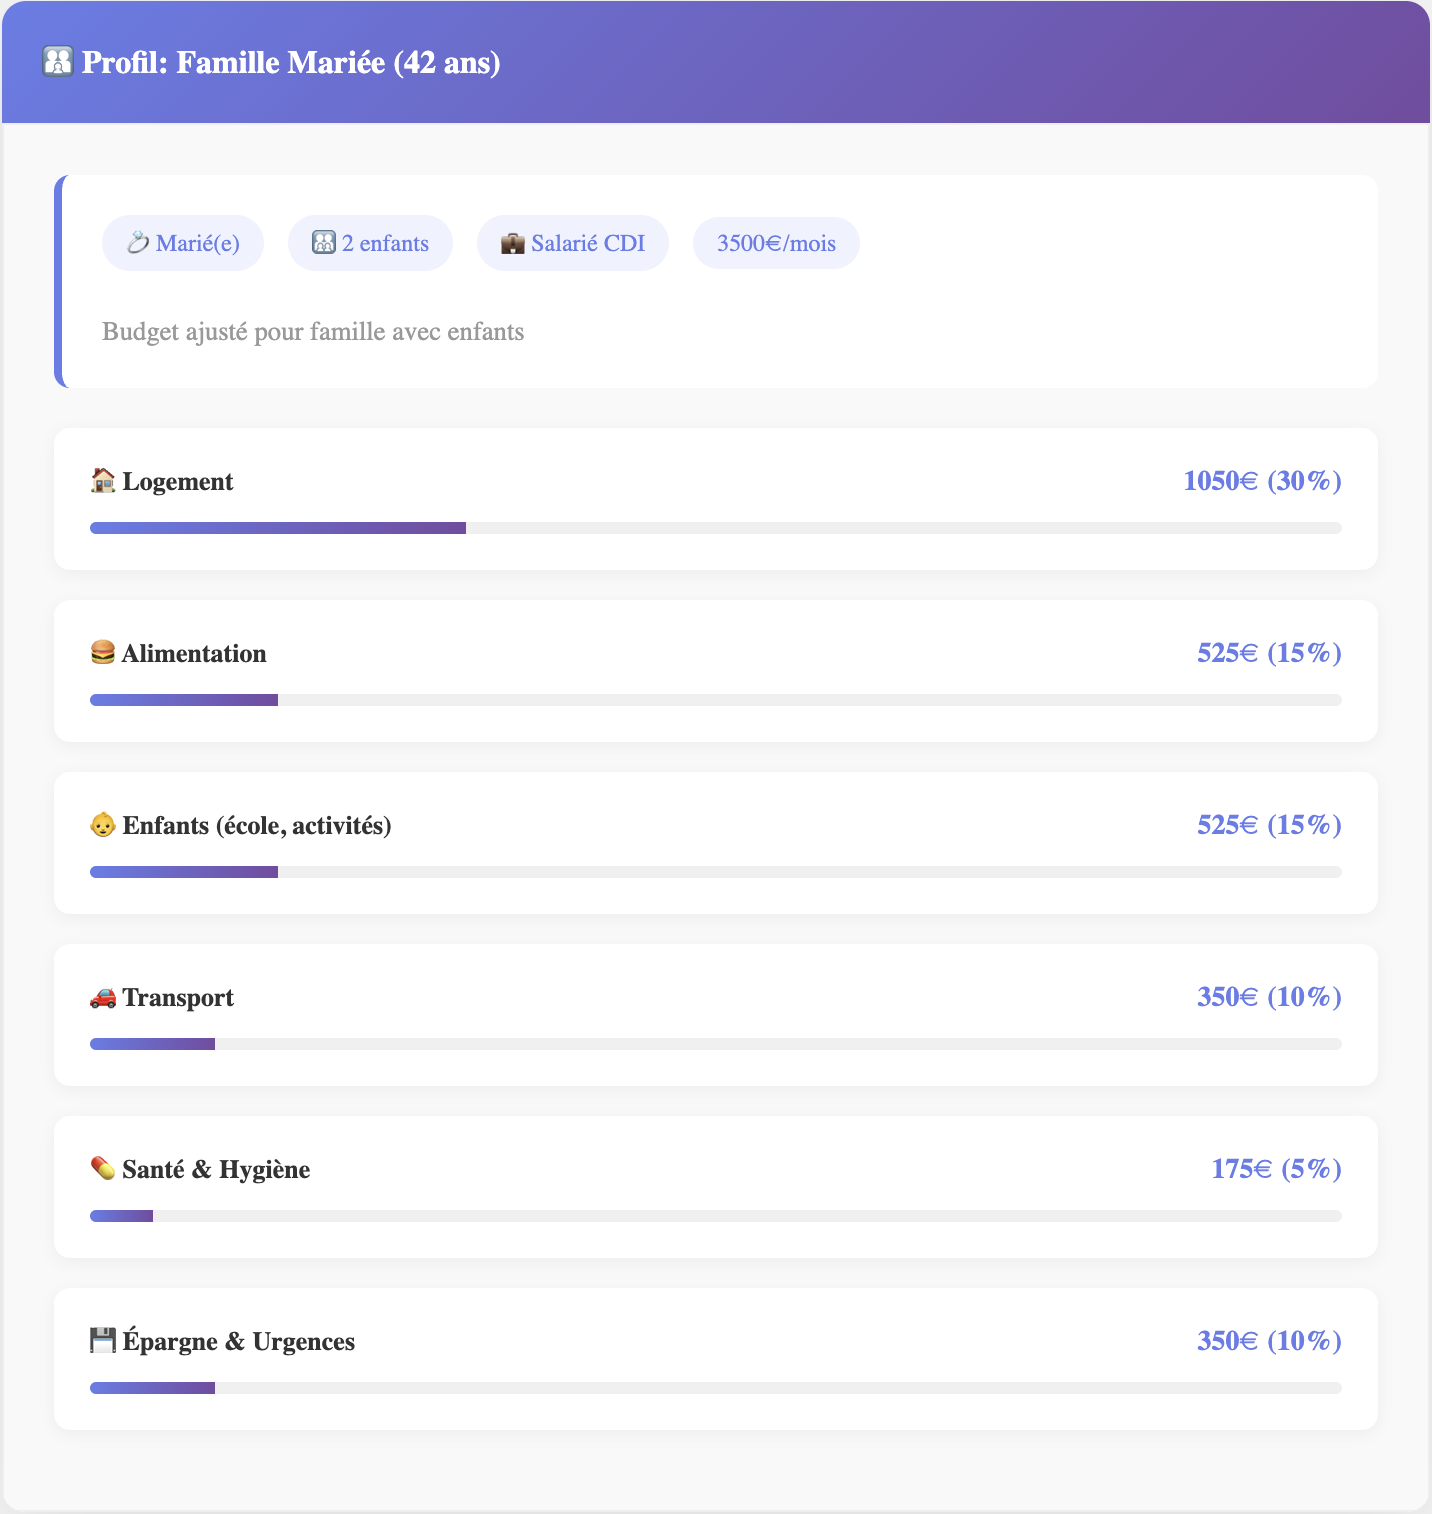
\includegraphics[width=\linewidth, height=0.68\textheight, keepaspectratio]{profil2.png}
    \end{column}
    \begin{column}{0.31\textwidth}
      \centering
      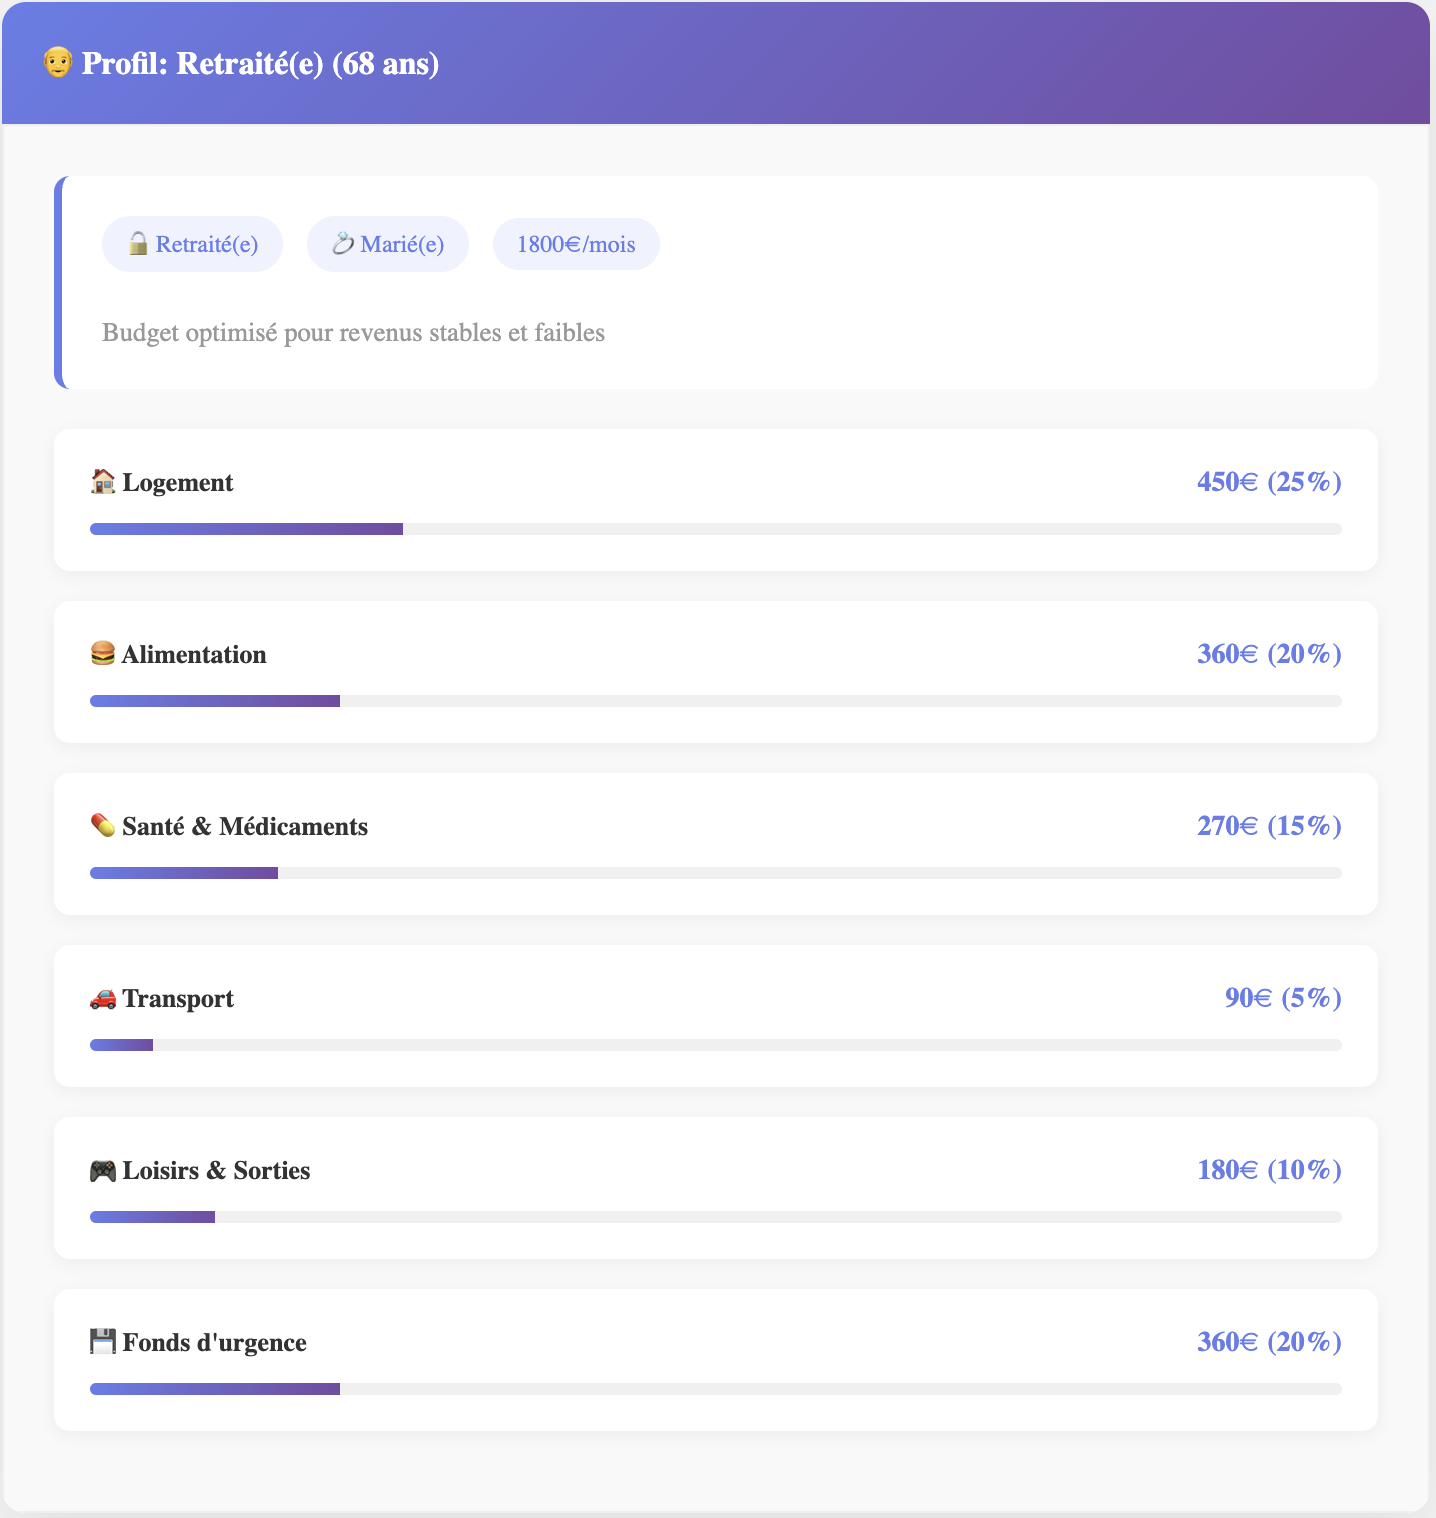
\includegraphics[width=\linewidth, height=0.68\textheight, keepaspectratio]{profil3.png}
    \end{column}
  \end{columns}
  \vspace{0.2cm}
  \centering\small Questionnaire rempli à l'inscription → personnalisation des conseils et des seuils d'alerte
\end{frame}

\begin{frame}{Priorisation des besoins — Méthode MoSCoW}
  \begin{columns}[t]
    \begin{column}{0.48\textwidth}
      \begin{alertblock}{\faCheckDouble\ Must Have}
        \begin{itemize}
          \item Authentification sécurisée (JWT)
          \item CRUD Transactions
          \item Enveloppes Budgétaires
          \item Dashboard Synthétique
        \end{itemize}
      \end{alertblock}
      \vspace{0.3cm}
      \begin{block}{Should Have}
        \begin{itemize}
          \item Export données (RGPD)
          \item Objectifs d'épargne
          \item Notifications de seuils
        \end{itemize}
      \end{block}
    \end{column}
    \begin{column}{0.48\textwidth}
      \begin{block}{Could Have}
        \begin{itemize}
          \item Conseils personnalisés
          \item Mode sombre
          \item Rapports PDF mensuels
        \end{itemize}
      \end{block}
      \vspace{0.3cm}
      \begin{block}{Won't Have (V1)}
        \begin{itemize}
          \item Agrégation bancaire automatique
          \item Application mobile native
        \end{itemize}
      \end{block}
    \end{column}
  \end{columns}
\end{frame}

% ═════════════════════════════════════════════════════════════════════════
\section{Maquettage}
% ═════════════════════════════════════════════════════════════════════════

\fullimg{diagramme_context.png}{Diagramme de contexte}

\fullimg{cas-utilisation.png}{Diagramme de cas d'utilisation}

\begin{frame}{Zoning Desktop}
  \begin{center}
    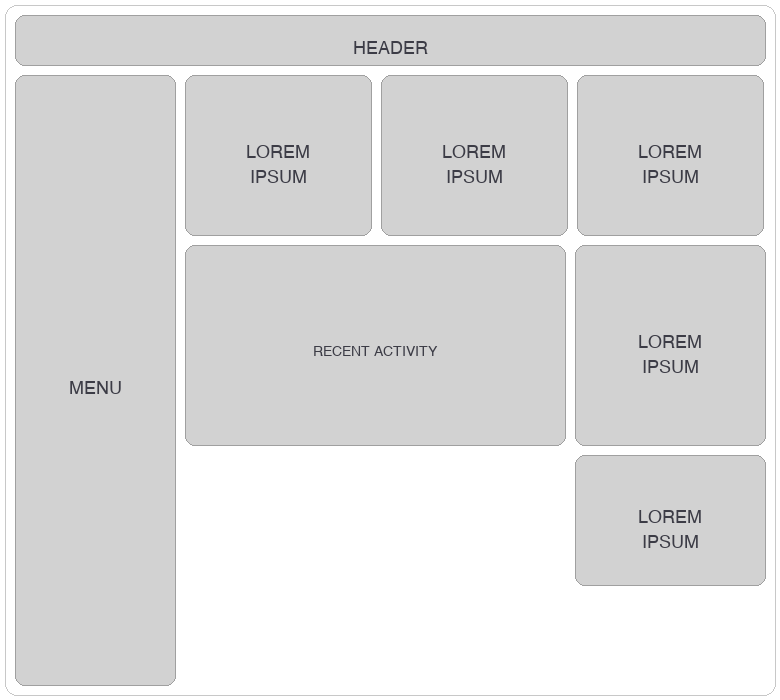
\includegraphics[max width=\linewidth, max height=0.82\textheight, keepaspectratio]{zoning-desktop.png}
  \end{center}
\end{frame}

\begin{frame}{Zoning — Page d'inscription}
  \begin{center}
    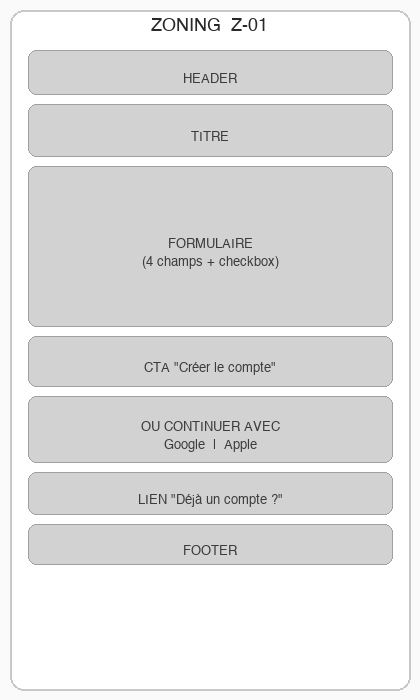
\includegraphics[max width=\linewidth, max height=0.82\textheight, keepaspectratio]{zoning-register.png}
  \end{center}
\end{frame}

\begin{frame}{Zoning Dashboard Mobile}
  \begin{center}
    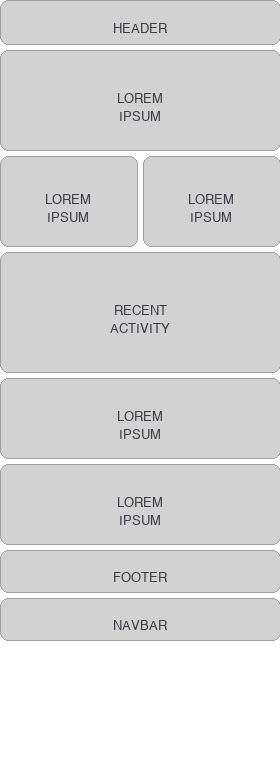
\includegraphics[max width=0.5\linewidth, max height=0.82\textheight, keepaspectratio]{zoning-dashboard-mobile.png}
  \end{center}
\end{frame}

\begin{frame}{Wireframe — Page d'inscription}
  \begin{center}
    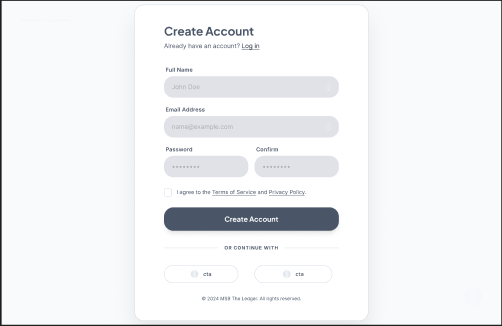
\includegraphics[max width=\linewidth, max height=0.82\textheight, keepaspectratio]{wireframe-register.png}
  \end{center}
\end{frame}

\begin{frame}{Wireframe — Dashboard Desktop}
  \begin{center}
    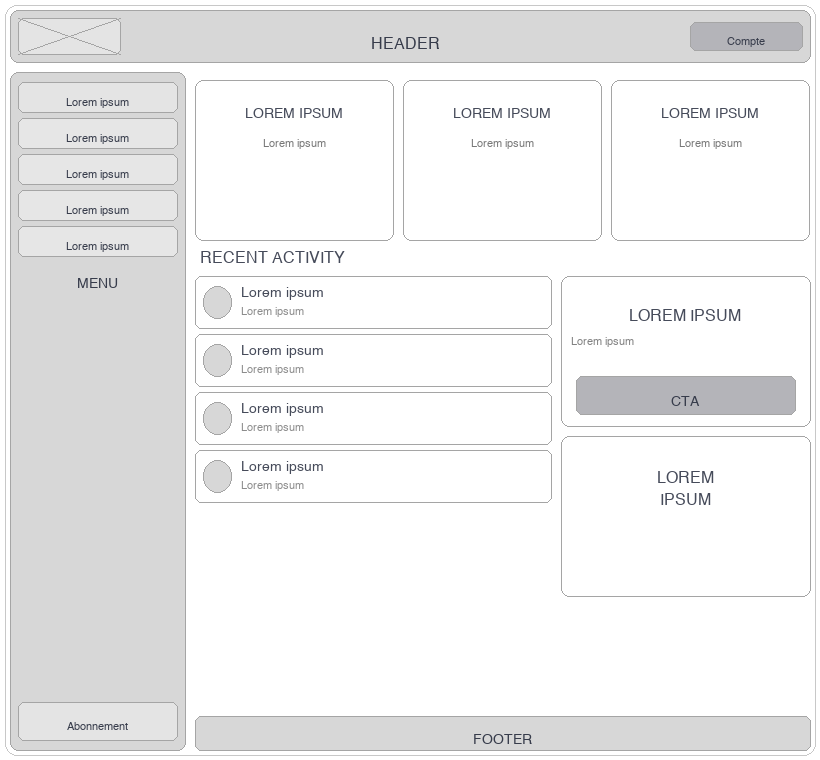
\includegraphics[max width=\linewidth, max height=0.82\textheight, keepaspectratio]{wireframe-dashboard-desktop.png}
  \end{center}
\end{frame}

\begin{frame}{Wireframe — Dashboard Mobile}
  \begin{center}
    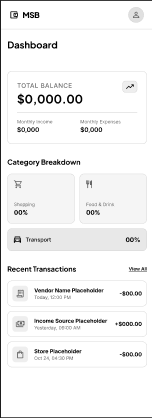
\includegraphics[max width=0.5\linewidth, max height=0.82\textheight, keepaspectratio]{wireframe-dashboard-mobile.png}
  \end{center}
\end{frame}

% ═════════════════════════════════════════════════════════════════════════
\section{Architecture logicielle}
% ═════════════════════════════════════════════════════════════════════════

\fullimg{arch-3tiers-app-budget-v3.png}{Architecture 3-Tiers}

\fullimg{diagramme-packages.png}{Diagramme de packages}

\fullimg{seq-auth-login.png}{Diagramme de séquence : Authentification}

\fullimg{seq-create-transaction.png}{Diagramme de séquence : Création de transaction}

\fullimg{seq-budget-alert.png}{Diagramme de séquence : Alerte budgétaire}

\fullimg{class-diagram-app-budget-v3.png}{Diagramme de classes}

% ═════════════════════════════════════════════════════════════════════════
\section{Base de données}
% ═════════════════════════════════════════════════════════════════════════

\begin{frame}{Méthode Merise — démarche de modélisation}
  \begin{columns}[c]
    \begin{column}{0.3\textwidth}
      \centering
      \begin{block}{\centering MCD}
        \centering\small Modèle Conceptuel\\
        Entités et associations\\cardinalités 1,N / 0,N
      \end{block}
    \end{column}
    \begin{column}{0.06\textwidth}
      \centering\Large$\Rightarrow$
    \end{column}
    \begin{column}{0.3\textwidth}
      \centering
      \begin{block}{\centering MLD}
        \centering\small Modèle Logique\\
        Tables + clés étrangères\\relations FK
      \end{block}
    \end{column}
    \begin{column}{0.06\textwidth}
      \centering\Large$\Rightarrow$
    \end{column}
    \begin{column}{0.3\textwidth}
      \centering
      \begin{block}{\centering MPD}
        \centering\small Modèle Physique\\
        Types SQL, contraintes\\PostgreSQL 15
      \end{block}
    \end{column}
  \end{columns}
  \vspace{0.5cm}
  \begin{alertblock}{Tables PostgreSQL}
    \centering\small
    \texttt{users} · \texttt{transactions} · \texttt{budgets} · \texttt{objectifs} · \texttt{user\_profiles} · \texttt{reports}
  \end{alertblock}
\end{frame}

\fullimg{mcd-app-budget-v3.png}{Modèle Conceptuel de Données (MCD)}

\fullimg{mld-app-budget.png}{Modèle Logique de Données (MLD)}

\fullimg{mpd-app-budget.png}{Modèle Physique de Données (MPD)}

% ═════════════════════════════════════════════════════════════════════════
\section{Accès aux données SQL \& NoSQL}
% ═════════════════════════════════════════════════════════════════════════

\begin{frame}{PostgreSQL — Données structurées}
  \begin{columns}[t]
    \begin{column}{0.48\textwidth}
      \begin{block}{Connexion \& requêtes}
        \begin{itemize}
          \item \textbf{pg-promise} : connexion poolée
          \item Requêtes paramétrées \texttt{\$1, \$2...}\\$\rightarrow$ protection anti-injection SQL
          \item Transactions ACID pour opérations critiques
        \end{itemize}
      \end{block}
    \end{column}
    \begin{column}{0.48\textwidth}
      \begin{block}{Optimisations}
        \begin{itemize}
          \item Index composites \texttt{user\_id + date}\\$\rightarrow$ gain 60\% sur P95
          \item Pagination côté serveur (limit 50)
          \item Compression gzip (réduction 70\% payload)
        \end{itemize}
      \end{block}
    \end{column}
  \end{columns}
  \vspace{0.4cm}
  \begin{alertblock}{Sécurité}
    \centering bcrypt (hachage mots de passe) \quad·\quad JWT accessToken 15 min + refreshToken 7 j \quad·\quad Cookies HTTPOnly
  \end{alertblock}
\end{frame}

\begin{frame}{MongoDB — Données documentaires}
  \begin{columns}[t]
    \begin{column}{0.48\textwidth}
      \begin{block}{Rôle dans l'application}
        \begin{itemize}
          \item Stockage des \textbf{snapshots de rapports PDF}
          \item Modèle Mongoose \texttt{Report}
          \item Données agrégées sous forme JSON
          \item Lien avec PostgreSQL via \texttt{userId}
        \end{itemize}
      \end{block}
    \end{column}
    \begin{column}{0.48\textwidth}
      \begin{block}{Pattern dual-DB}
        \begin{itemize}
          \item \textbf{PostgreSQL} → données structurées transactionnelles
          \item \textbf{MongoDB} → documents flexibles (rapports)
          \item Suppression RGPD synchronisée sur les deux BDD
        \end{itemize}
      \end{block}
    \end{column}
  \end{columns}
  \vspace{0.4cm}
  \begin{block}{RGPD — Droits utilisateur}
    \centering\small
    Art.15 Export · Art.16 Modification · Art.17 Suppression · Art.20 Portabilité
  \end{block}
\end{frame}

% ═════════════════════════════════════════════════════════════════════════
\section{Bilan}
% ═════════════════════════════════════════════════════════════════════════

\begin{frame}{Bilan — Compétences couvertes}
  \begin{columns}[t]
    \begin{column}{0.48\textwidth}
      \begin{block}{\faCheckCircle\ Compétences validées}
        \begin{itemize}
          \item \textbf{Analyser les besoins et maquetter}\\
                \textcolor{gray}{\small MoSCoW · Use Cases · Wireframes · Zoning}
          \vspace{0.15cm}
          \item \textbf{Définir l'architecture logicielle}\\
                \textcolor{gray}{\small 3-Tiers · Packages · Séquence · Classes}
          \vspace{0.15cm}
          \item \textbf{Concevoir une BDD relationnelle}\\
                \textcolor{gray}{\small Merise : MCD $\to$ MLD $\to$ MPD · PostgreSQL}
          \vspace{0.15cm}
          \item \textbf{Développer les composants d'accès}\\
                \textcolor{gray}{\small SQL (pg-promise) · NoSQL (Mongoose)}
        \end{itemize}
      \end{block}
    \end{column}
    \begin{column}{0.48\textwidth}
      \begin{block}{\faCogs\ Pratiques appliquées}
        \begin{itemize}
          \item Agile Scrum — 4 sprints de 2 semaines
          \item CI/CD GitHub Actions
          \item Tests de performance k6 (50 VU)
          \item Sécurité RGPD (art. 15, 16, 17, 20)
          \item Application déployée et fonctionnelle
        \end{itemize}
      \end{block}
      \vspace{0.3cm}
      \begin{alertblock}{\centering Résultat}
        \centering\small
        Cycle complet couvert :\\
        Besoins $\to$ Maquette $\to$ Architecture\\
        $\to$ BDD $\to$ Développement $\to$ Tests
      \end{alertblock}
    \end{column}
  \end{columns}
\end{frame}

% ── FIN ──────────────────────────────────────────────────────────────────
{
\setbeamertemplate{footline}{}
\begin{frame}
  \begin{tikzpicture}[remember picture,overlay]
    \fill[primary] (current page.north west) rectangle (current page.south east);
    \fill[secondary!50,opacity=0.25] (current page.north east) circle (7cm);
    \fill[accent!40,opacity=0.18] (current page.south west) circle (5cm);
  \end{tikzpicture}
  \vspace{1.5cm}
  \begin{center}
    {\Huge\textbf{\textcolor{white}{Merci pour votre attention}}}\\[0.8cm]
    {\LARGE\textcolor{accent}{Questions ?}}\\[1.2cm]
    {\large\textcolor{white!85}{Abdelghani Saidi — PFE 2026}}\\[0.3cm]
    {\normalsize\textcolor{white!65}{My Smart Budget — Application web de gestion budgétaire}}
  \end{center}
\end{frame}
}

\end{document}
